%\documentclass[12pt]{report} 
%\begin{document}

\chapter*{Dodatak: Prikaz aktivnosti grupe}
		\addcontentsline{toc}{chapter}{Dodatak: Prikaz aktivnosti grupe}
		
		\section*{Dnevnik sastajanja}
		
		\begin{packed_enum}
			\item  sastanak
			
			\item[] \begin{packed_item}
				\item Datum: 5. listopada 2020. 
				\item Prisustvovali:  Igor Stančin, svi članovi tima
				\item Teme sastanka:
				\begin{packed_item}
					\item  Uvodni sastanak s asistentom
				\end{packed_item}
			\end{packed_item}
			
			\item  sastanak
			\item[] \begin{packed_item}
				\item Datum: 7. listopada 2020. 
				\item Prisustvovali: svi članovi tima
				\item Teme sastanka:
				\begin{packed_item}
					\item  upoznavanje
					\item  dogovor o tehnologijama
				\end{packed_item}
			\end{packed_item}
			
			\item  sastanak
			\item[] \begin{packed_item}
				\item Datum: 12. listopada 2020. 
				\item Prisustvovali: Igor Stančin, Ivan Klabučar, Petar Gabrijel Kedmenec
				\item Teme sastanka:
				\begin{packed_item}
					\item  pitanja oko funkcionalnih zahtjeva
				\end{packed_item}
			\end{packed_item}
			
			\item  sastanak
			\item[] \begin{packed_item}
				\item Datum: 15. listopada 2020. 
				\item Prisustvovali: svi članovi tima
				\item Teme sastanka:
				\begin{packed_item}
					\item  raspodjela poslova oko obrazaca uporabe
				\end{packed_item}
			\end{packed_item}
			
			\item  sastanak
			\item[] \begin{packed_item}
				\item Datum: 21. listopada 2020. 
				\item Prisustvovali: svi članovi tima
				\item Teme sastanka:
				\begin{packed_item}
					\item  raspodjela poslova oko UML dijagrama
					\item  rasprava o prirodi uloge Admin
				\end{packed_item}
			\end{packed_item}
		
			\item  sastanak
			\item[] \begin{packed_item}
				\item Datum: 24. listopada 2020. 
				\item Prisustvovali: Ivan Klabučar, Fran Leontić, Luka Žižić
				\item Teme sastanka:
				\begin{packed_item}
					\item  raspravljanje o implementaciji dnevnih taktika
				\end{packed_item}
			\end{packed_item}
			
			\item  sastanak
			\item[] \begin{packed_item}
				\item Datum: 24. listopada 2020. 
				\item Prisustvovali: Ivan Klabučar, Petar Gabrijel Kedmenec
				\item Teme sastanka:
				\begin{packed_item}
					\item  rješavanje konflikata na GitLabu
				\end{packed_item}
			\end{packed_item}
		
			\item  sastanak
			\item[] \begin{packed_item}
				\item Datum: 26. listopada 2020. 
				\item Prisustvovali: Igor Stančin, svi članovi tima
				\item Teme sastanka:
				\begin{packed_item}
					\item  razjašnjavanje dijagrama obrazaca i sekvencijskih dijagrama
				\end{packed_item}
			\end{packed_item}
			
			\item  sastanak
			\item[] \begin{packed_item}
				\item Datum: 29. listopada 2020. 
				\item Prisustvovali: svi članovi tima
				\item Teme sastanka:
				\begin{packed_item}
					\item  raspodjela kodiranja
				\end{packed_item}
				\item Zaključci:
				\begin{packed_item}
					\item Ivar Cmrečak, Fran Leontić i Ivan Klabučar rade na bazi
					\item Petar Gabrijel Kedmenec i Luka Žižić rade na uspostavljanju templatea za listanje dnevnih taktika
					\item Mihael Svetec i Sven Paprskar rade na uspostavljanju templatea za listanje novosti
				\end{packed_item}
			\end{packed_item}
		
			\item  sastanak
			\item[] \begin{packed_item}
				\item Datum: 31. listopada 2020. 
				\item Prisustvovali: Ivan Klabučar, Fran Leontić, Luka Žižić, Ivar Cmrečak
				\item Teme sastanka:
				\begin{packed_item}
					\item  raspravljanje o tablicama u bazi podataka
				\end{packed_item}
			\end{packed_item}

		\eject 
			\item  sastanak
			\item[] \begin{packed_item}
				\item Datum: 4. studenoga 2020. 
				\item Prisustvovali: svi članovi tima
				\item Teme sastanka:
				\begin{packed_item}
					\item  raspravljanje o implementaciji potrebnih funkcija za demonstraciju generičke funkcionalnosti
				\end{packed_item}
			\end{packed_item}
		
			\item  sastanak
			\item[] \begin{packed_item}
				\item Datum: 9. studenoga 2020. 
				\item Prisustvovali: Igor Stančin, svi članovi tima
				\item Teme sastanka:
				\begin{packed_item}
					\item pokazivanje generičke funkcionalnosti aplikacije
					\item pregled dokumentacije
				\end{packed_item}
			\end{packed_item}
			
			\item  sastanak
			\item[] \begin{packed_item}
				\item Datum: 11. studenoga 2020. 
				\item Prisustvovali: Ivan Klabučar, Ivar Cmrečak, Petar Gabrijel Kedmenec, Fran Leontić, Mihael Svetec, Sven Paprskar
				\item Teme sastanka:
				\begin{packed_item}
					\item raspodjela uloga prije pauze za međuispite
				\end{packed_item}
				\item Zaključci:
				\begin{packed_item}
					\item Petar Gabrijel Kedmenec dovršava uređenje dokumentacije za prvu predaju
					\item Sven Paprskar izrađuje template za prikaz transakcija
					\item Luka Žižić izrađuje template za dodavanje novih obavijesti
					\item Mihael Svetec izrađuje template za dodavanje, listanje i prijavljivanje na treninge
					\item Fran Leontić izrađuje template za prikaz korisničkog profila
					\item Ivan Klabučar izrađuje template za objavu treninga
					\item Ivar Cmrečak uspostavlja bazu podataka
				\end{packed_item}
			\end{packed_item}
			
			\item  sastanak
			\item[] \begin{packed_item}
				\item Datum: 18. studenoga 2020. 
				\item Prisustvovali: svi članovi tima
				\item Teme sastanka:
				\begin{packed_item}
					\item  pregled napravljenog i komentiranje o potrebnim ispravcima programskog koda
				\end{packed_item}
			\end{packed_item}
			\eject
			\item  sastanak
			\item[] \begin{packed_item}
				\item Datum: 25. studenoga 2020. 
				\item Prisustvovali: svi članovi tima
				\item Teme sastanka:
				\begin{packed_item}
					\item  daljnja podjela rada vezana uz kodiranje i dokumentaciju
				\end{packed_item}
			\end{packed_item}
			
			\item  sastanak
			\item[] \begin{packed_item}
				\item Datum: 2. prosinca 2020. 
				\item Prisustvovali: svi članovi tima
				\item Teme sastanka:
				\begin{packed_item}
					\item  razrješavanje problema vezanog uz programiranje
				\end{packed_item}
			\end{packed_item}
			
			\item  sastanak
			\item[] \begin{packed_item}
				\item Datum: 9. prosinca 2020. 
				\item Prisustvovali: svi članovi tima
				\item Teme sastanka:
				\begin{packed_item}
					\item  analiza dosadašnjeg rada, dogovor o nastavku rada
				\end{packed_item}
			\end{packed_item}
			
			\item  sastanak
			\item[] \begin{packed_item}
				\item Datum: 14. prosinca 2020. 
				\item Prisustvovali: svi članovi tima
				\item Teme sastanka:
				\begin{packed_item}
					\item  dokumentacija, raspravljanje parova koji rade na zajedničkom problemu
				\end{packed_item}
			\end{packed_item}
			
			\item  sastanak
			\item[] \begin{packed_item}
				\item Datum: 18. prosinca 2020. 
				\item Prisustvovali: svi članovi tima
				\item Teme sastanka:
				\begin{packed_item}
					\item  dogovor o nastavku rada na dokumentaciji i programskim rješenjima
				\end{packed_item}
			\end{packed_item}
			
			\item  sastanak
			\item[] \begin{packed_item}
				\item Datum: 23. prosinca 2020. 
				\item Prisustvovali: svi članovi tima
				\item Teme sastanka:
				\begin{packed_item}
					\item  podjela posla preko zimskih praznika
				\end{packed_item}
			\end{packed_item}
		
		\item  sastanak
		\item[] \begin{packed_item}
			\item Datum: 4. siječnja 2021. 
			\item Prisustvovali: svi članovi tima
			\item Teme sastanka:
			\begin{packed_item}
				\item dogovori oko završavanja programiranja vezanog uz alfa verziju aplikacije
			\end{packed_item}
		\end{packed_item}
			
			\item  sastanak
			\item[] \begin{packed_item}
				\item Datum: 4. siječnja 2021. 
				\item Prisustvovali: Igor Stančin, svi članovi tima
				\item Teme sastanka:
				\begin{packed_item}
					\item prezentacija alfa inačice aplikacije asistentu Igoru Stančinu
				\end{packed_item}
			\end{packed_item}
		\end{packed_enum}
		
		\eject
		\section*{Tablica aktivnosti}
		
			\textbf{\textit{Kontinuirano osvježavanje}}\\
			
			 \textit{Napomena: Doprinose u aktivnostima treba navesti u satima po članovima grupe po aktivnosti.}
					
						
			
			\begin{longtabu} to \textwidth {|X[7, l]|X[1, c]|X[1, c]|X[1, c]|X[1, c]|X[1, c]|X[1, c]|X[1, c]|}
								
				\cline{2-8} \multicolumn{1}{c|}{\textbf{}} &     \multicolumn{1}{c|}{\rotatebox{90}{\textbf{Ivar Cmrečak}}} & \multicolumn{1}{c|}{\rotatebox{90}{\textbf{Sven Paprskar }}} &	\multicolumn{1}{c|}{\rotatebox{90}{\textbf{Ivan Klabučar}}} &	\multicolumn{1}{c|}{\rotatebox{90}{\textbf{Mihael Svetec }}} &
				\multicolumn{1}{c|}{\rotatebox{90}{\textbf{Fran Leontić }}} &
				\multicolumn{1}{c|}{\rotatebox{90}{\textbf{Petar Gabrijel Kedmenec }}} &	\multicolumn{1}{c|}{\rotatebox{90}{\textbf{Luka Žižić }}} \\ \hline 
				\endfirsthead
				
			
				\cline{2-8} \multicolumn{1}{c|}{\textbf{}} &     \multicolumn{1}{c|}{\rotatebox{90}{\textbf{Ivar Cmrečak}}} & \multicolumn{1}{c|}{\rotatebox{90}{\textbf{Sven Paprskar }}} &	\multicolumn{1}{c|}{\rotatebox{90}{\textbf{Ivan Klabučar}}} &
				\multicolumn{1}{c|}{\rotatebox{90}{\textbf{Mihael Svetec }}} &	\multicolumn{1}{c|}{\rotatebox{90}{\textbf{Fran Leontić }}} &
				\multicolumn{1}{c|}{\rotatebox{90}{\textbf{Petar Gabrijel Kedmenec }}} &	\multicolumn{1}{c|}{\rotatebox{90}{\textbf{Luka Žižić }}} \\ \hline 
				\endhead
				
				
				\endfoot
							
				 
				\endlastfoot
				
				Upravljanje projektom 		& 10 &  & 12 &  &  &  & \\ \hline
				Opis projektnog zadatka 	&  & 1 & 1 &  & 2.5  &  & 2\\ \hline
				
				Funkcionalni zahtjevi       &  & 1 &  &  &  & 3 &  \\ \hline
				Opis pojedinih obrazaca 	& 1 & 2 & 1 & 3 &  & 3 & \\ \hline
				Dijagram obrazaca 			&  & 1 &  & 2 &  &  & \\ \hline
				Sekvencijski dijagrami 		&  &  & 3 &  & 1.5 &  & 2.5\\ \hline
				Opis ostalih zahtjeva 		&  &  &  &  &  & 1.5 &  \\ \hline

				Arhitektura i dizajn sustava	 & 1 &  &  &  &  &  &  \\ \hline
				Baza podataka				& 1 &  & 2 & 1 & 2 & 1 & 1 \\ \hline
				Dijagram razreda 			&  &  & 5 &  & 1 &  &   \\ \hline
				Dijagram stanja				&  & 5 &  &  &  &  &  \\ \hline
				Dijagram aktivnosti 		&  & 2 &  &  &  &  &  \\ \hline
				Dijagram komponenti			&  &  &  &  &  &  &  \\ \hline
				Korištene tehnologije i alati 		& 2 & 2 &  &  &  &  &  \\ \hline
				Ispitivanje programskog rješenja 	&  & 2 & 1 & 1 &  &  &  \\ \hline
				Dijagram razmještaja			&  & 1.5 &  &  &  &  &  \\ \hline
				Upute za puštanje u pogon 		&  & 1.5 &  &  &  &  &  \\ \hline 
				Dnevnik sastajanja 			&  & 1 & .5 &  &  & 1 &  \\ \hline
				Zaključak i budući rad 		&  & 1 &  &  &  &  &  \\  \hline
				Popis literature 			&  &  &  &  &  & .5 &  \\  \hline
				&  &  &  &  &  &  &  \\ \hline \hline
				Izrada baze podataka 		& 3 &  & 3 &  &  &  & \\ \hline 
				Spajanje s bazom podataka 		& 3 &  &  &  &  &  &  \\ \hline
				Izrada frontenda 			& 3 &  & 6 &  & 2  &  &  \\  \hline
				Izrada autorizacije 			& 3 &  &  &  &  &  & \\  \hline
				Izrada stranice s novostima 			&  & 2 &  & 2 &  &  & 5 \\  \hline
				Izrada stranice s dnevnim taktikama 		&  &  & 6 &  &  & 2 & 3 \\  \hline
				Izrada stranice s treninzima 		&  &  &  & 5 &  &  &  \\ \hline
				Izrada stranice s turnirima 		&  &  &  & 5 &  &  &  \\ \hline
				Izrada početne stranice i nav-bara 		&  &  &  & 2 &  &  & 0.5 \\ \hline
				Izrada stranice s dojavama pogreški 		&  &  &  & 3 &  &  &  \\ \hline
				Izrada stranice profila		&  &  &  &  & 5 &  &  \\ \hline
				Izrada liste profila i detaljnog prikaza		&  &  &  &  & 4 &  &  \\ \hline
				Izrada stranice za plaćanje članarine 		&  &  &  &  &  &  & 3 \\ \hline
				Izrada adminove liste neplaćenh članarina		&  &  &  &  & 2 & 1 &  \\ \hline
				Izrada adminove liste svih transakcija &  &  &  &  &  & 4 &  \\ \hline
				Izrada rang liste &  &  & 3 &  &  & 1 &  \\ \hline
				Deployment na remote server & 4 &  &  &  &  &  &  \\ \hline
				
			\end{longtabu}
					
					
		\eject
		\section*{Dijagrami pregleda promjena}
		
		\begin{figure}[H]
			\centerfloat
			\advance\leftskip0.5cm
			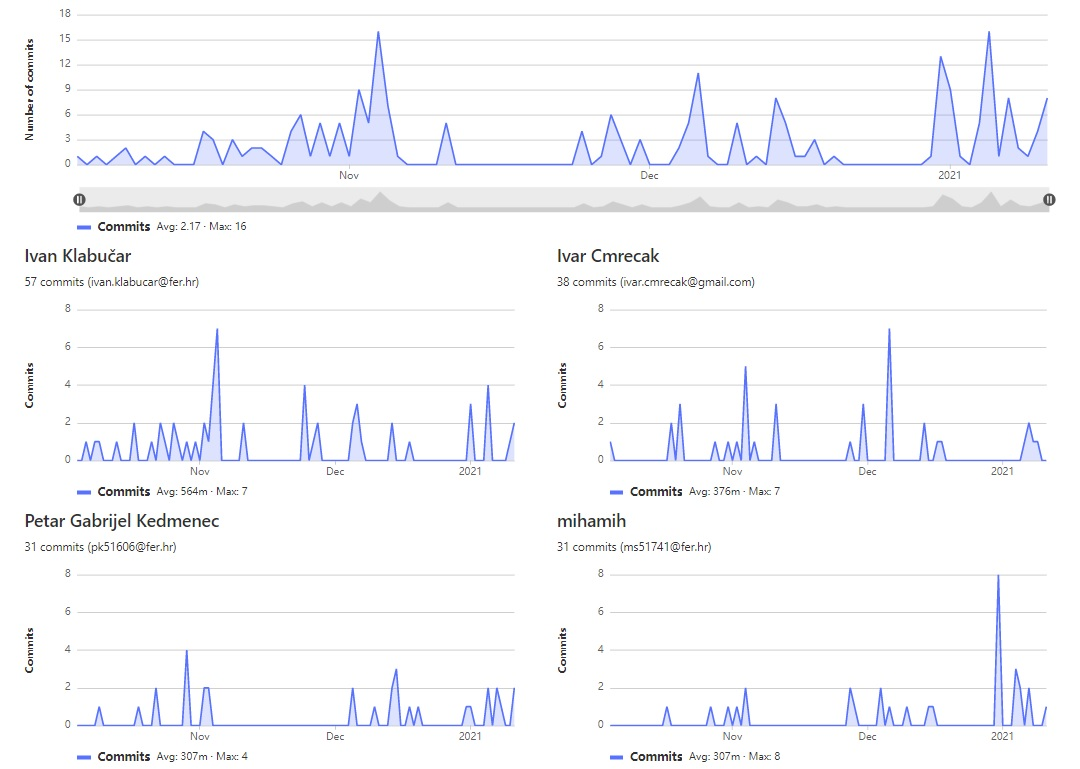
\includegraphics[scale=0.60]{slike/dijpregprom1.jpg} %veličina slike u odnosu na originalnu datoteku i pozicija slike
			\caption{Prikaz aktivnosti na repozitoriju 1. dio}
		\end{figure}
	
	\begin{figure}[H]
		\centerfloat
		\advance\leftskip0.5cm
		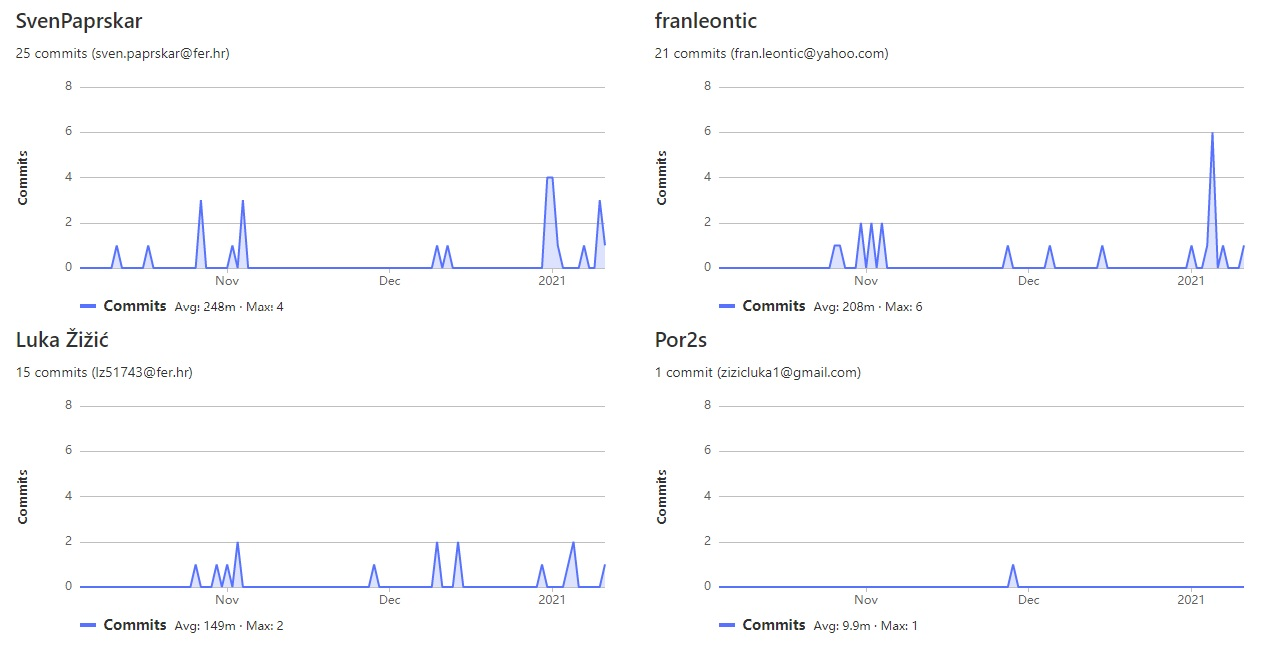
\includegraphics[scale=0.55]{slike/dijpregprom2.jpg} %veličina slike u odnosu na originalnu datoteku i pozicija slike
		\caption{Prikaz aktivnosti na repozitoriju 2. dio}
	\end{figure}
		
	\end{document}